\let\negmedspace\undefined
\let\negthickspace\undefined
\documentclass[journal]{IEEEtran}
\usepackage[a5paper, margin=10mm, onecolumn]{geometry}
%\usepackage{lmodern} % Ensure lmodern is loaded for pdflatex
\usepackage{tfrupee} % Include tfrupee package

\setlength{\headheight}{1cm} % Set the height of the header box
\setlength{\headsep}{0mm}     % Set the distance between the header box and the top of the text

\usepackage{gvv-book}
\usepackage{gvv}
\usepackage{cite}
\usepackage{amsmath,amssymb,amsfonts,amsthm}
\usepackage{algorithmic}
\usepackage{graphicx}
\usepackage{textcomp}
\usepackage{xcolor}
\usepackage{txfonts}
\usepackage{listings}
\usepackage{enumitem}
\usepackage{mathtools}
\usepackage{gensymb}
\usepackage{comment}
\usepackage[breaklinks=true]{hyperref}
\usepackage{tkz-euclide} 
\usepackage{listings}
% \usepackage{gvv}                                        
\def\inputGnumericTable{}                                 
\usepackage[latin1]{inputenc}                                
\usepackage{color}                                            
\usepackage{array}                                            
\usepackage{longtable}                                       
\usepackage{calc}                                             
\usepackage{multirow}                                         
\usepackage{hhline}                                           
\usepackage{ifthen}                                           
\usepackage{lscape}
\begin{document}

\bibliographystyle{IEEEtran}
\vspace{3cm}

\title{
1-Vector Arithmetic \\
\large EE1030:Matrix Theory
}
\author{Gajjarapu Satyanarayana\\AI24BTECH11009
}
% \maketitle
% \newpage
% \bigskip
{\let\newpage\relax\maketitle}

\renewcommand{\thefigure}{\theenumi}
\renewcommand{\thetable}{\theenumi}



\numberwithin{equation}{enumi}
\numberwithin{figure}{enumi}
\renewcommand{\thetable}{\theenumi}


\textbf{Question}:1.8.24\\
Find a relation between $x$ and $y$ such that the point ($x,y$) is equidistant from the points (7,1) and (3,5).
\\
\textbf{Solution:}
\renewcommand{\tablename}{Table 1.8.24.1}
\begin{table}[h!]
  \centering
  \begin{tabular}[12pt]{ |c| c|}
    \hline
    \textbf{Variables} & \textbf{Description}\\ 
    \hline
    $\textbf{V}_1, \vec{u}_1, f_1$ & Parameters of the parabola $y^2 = 4x$ \\
    \hline
     $\textbf{V}_2, \vec{u}_2, f_2$ & Parameters of the circle $4x^2 + 4xy^2 = 9$ \\
    \hline
    $\vec{x}^\intercal\brak{\textbf{V}_1 + \mu\textbf{V}_2}\vec{x} + 2\brak{\vec{u}_1 + \mu\vec{u}_2}^\intercal\vec{x} + \brak{f_1 + \mu f_2}$ & Intersection of two conics \\
    \hline
    \end{tabular}


  \caption{Labeling given coordinates as $\vec{A}$, $\vec{B}$, $\vec{C}$}
\end{table}
\\
$\vec{A}$ is said to be equidistant from $\vec{B}$ and $\vec{C}$ if 
 \begin{align}
	 \lVert \vec{B} - \vec{A} \rVert & = \lVert \vec{C} - \vec{A} \rVert \label{eq1.8.24.1} \\
	 \vec{B} - \vec{A} & = \myvec{7 \\ 1} - \myvec{x \\ y} \\ 
	 \vec{B} - \vec{A} & = \myvec{7 - x \\ 1 - y} \\ 
	 \brak{\vec{B} - \vec{A}}^\intercal & = \myvec{7 - x & 1 - y} \\ 
	 \vec{C} - \vec{A} & = \myvec{3 \\ 5} - \myvec{x \\ y} \\ 
	 \vec{C} - \vec{A} & = \myvec{3 - x \\ 5 - y} \\ 
	 \brak{\vec{C} - \vec{A}}^\intercal & = \myvec{3 - x & 5 - y}
 \end{align}
Given $\vec{A}$ is equidistant from $\vec{B}$ and $\vec{C}$, so $\lVert \vec{B} - \vec{A} \rVert = \lVert \vec{C} - \vec{A} \rVert$ from equation \ref{eq1.8.24.1} , \\
Therefore
\begin{align}
	\sqrt{\brak{\vec{B} - \vec{A}}^\intercal\brak{\vec{B} - \vec{A}}} & = \sqrt{\brak{\vec{C} - \vec{A}}^\intercal\brak{\vec{C} - \vec{A}}} \label{eq1.8.24.2}
\end{align}
Squaring the equation \ref{eq1.8.24.2} on both sides,
\begin{align}
	\brak{\vec{B} - \vec{A}}^\intercal\brak{\vec{B} - \vec{A}} & = \brak{\vec{C} - \vec{A}}^\intercal\brak{\vec{C} - \vec{A}} \\
	\myvec{7 - x & 1 - y}\myvec{7 - x \\ 1 - y} & = \myvec{3 - x & 5 - y}\myvec{3 - x \\ 5 - y} \\
	\brak{7 - x}^2 + \brak{1 - y}^2 & = \brak{3 - x}^2 + \brak{5 - y}^2 \\
	49 + x^2 - 14x + 1 + y^2 - 2y & = 9 + x^2 -6x + 25 + y^2 -10y \\
	8x - 8y - 16 & = 0 \\
	x - y - 2 & = 0
\end{align}
The relation between $x$ and $y$ is $x - y - 2 = 0.$
\begin{figure}[h!]
   \centering
   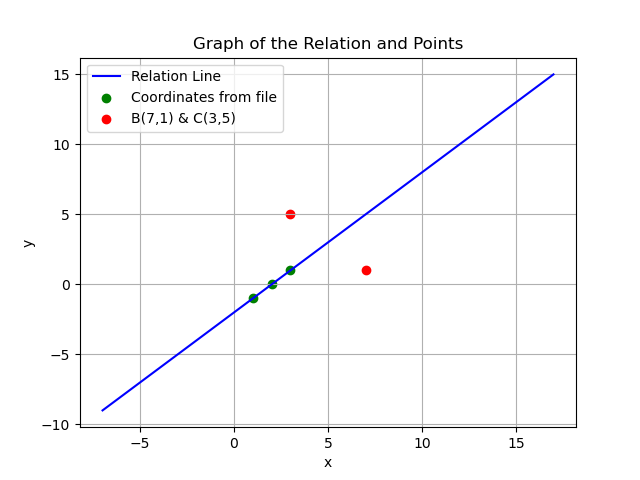
\includegraphics[width=0.7\linewidth]{figs/equi.png}
   \caption{Relation between $x$ and $y$: $x - y -2 = 0$}
   \end{figure}
   \end{document}
   
